\documentclass{amsart}
\usepackage{amsfonts, amsthm, amssymb, amsmath}
\usepackage{mathtools}
\usepackage{graphicx,caption,subcaption}
\usepackage{comment}
\usepackage{xcolor}
\usepackage{tikz}
%\usetikzlibrary{decorations.markings,arrows.meta,calc,fit,quotes,cd,math,external}
\usetikzlibrary{
  matrix,
  arrows,
  arrows.meta,
  calc,
  fit,
  quotes,
  cd,
  math,
  external,
  shapes,
  decorations.markings,
  decorations.pathreplacing,
  patterns,
  decorations.pathmorphing
}

\usepackage{url}
\usepackage[inline]{enumitem}
	\setlist{itemsep=0em, topsep=0em, parsep=0em}
	\setlist[enumerate]{label=(\alph*)}
\usepackage[all,2cell]{xy}\UseAllTwocells\SilentMatrices
\usepackage[breaklinks=true]{hyperref}%John's choices, can change; previous choice \definecolor{hyperrefcolor}{rgb}{0,0,0.7}
\definecolor{darkgreen}{rgb}{0,0.45,0}
\definecolor{myurlcolor}{rgb}{0.6,0,0}
\definecolor{mycitecolor}{rgb}{0,0,0.8}
\definecolor{myrefcolor}{rgb}{0,0,0.8}
\hypersetup{colorlinks, linkcolor=myrefcolor, citecolor=darkgreen, urlcolor=myurlcolor,
final,linktoc=page}
\usepackage[capitalize]{cleveref}
\crefname{equation}{}{}
\crefname{item}{}{}
\crefname{prop}{Proposition}{Propositions}

%
% environments and counters
%

\newtheorem{thm}{Theorem}[section]
\newtheorem{cnj}[thm]{Conjecture}
\newtheorem{lem}[thm]{Lemma}
\newtheorem{prop}[thm]{Proposition}
\newtheorem{cor}[thm]{Corollary}

\theoremstyle{remark}
	\newtheorem{remark}[thm]{Remark}
	\newtheorem{notation}[thm]{Notation}

\theoremstyle{definition}
	\newtheorem{ex}[thm]{Example} 
	\newtheorem{defn}[thm]{Definition}

% math text formatting
\newcommand{\cat}[1]{\mathsf{#1}}

% common category names

\newcommand{\Set}{\cat{Set}}
\newcommand{\Grph}{\cat{Grph}}
\newcommand{\Cat}{\cat{Cat}}
\newcommand{\twoCat}{\cat{2Cat}}
\newcommand{\Adj}{\cat{Adj}}
\newcommand{\one}{\mathbf{1}}
\newcommand{\two}{\mathbf{2}}
\newcommand{\Fib}{\cat{Fib}}
\newcommand{\OpFib}{\cat{OpFib}}
\newcommand{\Corefl}{\cat{Corefl}}
\newcommand{\Rali}{\cat{Rali}}

\newcommand{\C}{\cat{A}}
\newcommand{\D}{\cat{X}}
\newcommand{\A}{\cat{A}}
\newcommand{\X}{\cat{X}}
\newcommand{\U}{U}
\newcommand{\Q}{Q}
\renewcommand{\L}{L}
\newcommand{\R}{R}
\renewcommand{\P}{P}
\newcommand{\B}{\cat{B}}
\newcommand{\Y}{\cat{Y}}

\newcommand{\Cocart}{\mathrm{Cocart}}
\newcommand{\Cart}{\mathrm{Cart}}

\newcommand{\op}[1]{\operatorname{#1}}
\renewcommand{\t}[1]{\text{#1}}

\newcommand{\from}{\colon}
\newcommand{\xto}[1]{\xrightarrow{#1}}
\newcommand{\To}{\Rightarrow}
\newcommand{\Tto}{\Rrightarrow}
\newcommand{\bydef}{\coloneqq}
\newcommand{\define}{\textbf}%consider change to bold? or something else?

%
% math operators
%

\DeclareMathOperator{\Hom}{Hom}
\DeclareMathOperator{\id}{id}
\DeclareMathOperator{\ob}{Ob}
\DeclareMathOperator{\arr}{arr}
\DeclareMathOperator{\im}{im}
\DeclareMathOperator{\Aut}{Aut}
\DeclareMathOperator{\Bij}{Bij}
\DeclareMathOperator{\Sub}{Sub}
\DeclareMathOperator{\colim}{colim}
\newcommand{\iso}{\cong}

%
% tikz styles
%

% arrows for commuting diagram
\tikzset{
  cd/.style={
    ->,
    scale=6,
    >=angle 90,
    font=\scriptsize}
  }

% its us!

\definecolor{purple(x11)}{rgb}{0.5, 0.0, 0.5}
\newcommand{\chris}{\color{purple(x11)}}
\newcommand{\daniel}{\color{red}}


\begin{document}
\title{A note on Fibrations and Adjunctions}

\author{Daniel Cicala and Christina Vasilakopoulou} 
\address{Departement of Mathematics, University of California, Riverside, 900 University Avenue, 92521, USA}
\email{cicala@math.ucr.edu,vasilak@ucr.edu}

\begin{abstract}
Fibrations and Adjunctions rock.
\end{abstract}

\maketitle

\tableofcontents


\section{Introduction}

\begin{comment}
{\chris Christina's questions to Steve:}

I had a question regarding choice of (co)limits in categories. Please excuse my naivety, I haven't really gone into depths of such
questions before because I guess if one can avoid them, they tend to! But any insight or 'big picture' idea from you would be really,
really appreciated to help me understand better a situation I find myself in. In particular, feel free to correct me in the following
statements.

(1) 'Choosing limits' in a complete category amounts to choosing a specific (of the many isomorphic ones) adjoint to the
constant diagram functor. Therefore if a category has limits, we can assume it has chosen ones. Does this already require the axiom of
choice?

(2) Therefore this choice is already 'functorial'. However, can we 'choose the choice'? In particular, is it reasonable
to say that if C has pushouts for example, there is such a specific choice such that the pushout of f along the identity 'is'
exactly f (and the identity)?

(3) If a functor $F:C\to D$ between categories with pushouts preserves them in the ordinary sense, can we actually make a
choice of them in C and in D, such that F strictly preserves them? What assumptions should I make to be able to do that?
Or this is somehow extra, i.e. needs to be checked or required?

Thanks so much in advance for any intuition that would help wrap my head around these!

A quick question to end: it is a fact that every Grothendieck fibration is a particular case of Street fibration,
and I also read that every Street fibration factors as an equivalence of categories followed by a Grothendieck one.
(I am in the process of reading Street's paper, but) does this by any chance induce an equivalence of categories? Fib with StreetFib?

{\chris Steve's response:}

1. As you say, choosing limits amounts to choosing a specific adjoint to the diagonal functor (with corresponding
statements holding if you are using weighted limits). I certainly allow myself to regard a category with limits as having
chosen ones if I wish. I suppose from a formal point of view that does require the axiom of choice, but I also use this as necessary.
The category of sets does have a canonical choice, which means that many of the most commonly occurring complete categories
also have a canonical choice.

2. Functoriality is automatic, irrespective of choice issues. There is also no problem with first using the canonical
choice where it exists (for example with pushouts along identities) and then extending this arbitrarily to deal with other cases.
I guess that once again you need the axiom of choice for this, but are you actually worried about that?

3. I have never thought about this - at first sight it seems a bit unnatural. In any case, I think that this
is not automatic. Let $2={0->1}$ be the arrrow category, and let $C=2\times 2\times 2$ be the free-living commutative cube.
Each face of the cube is in fact a pushout; in fact C has a unique choice of pushouts. Let D be the category obtained from the
square $2\times 2$ by adding an extra object c isomorphic to (1,1). Then D contains two commutative squares:
the original 2x2, and one using the new object. This category once again has pushouts, but now there are choices to make.
There is an evident (unique) functor f:C->D sending the top face of the cube to the first square and the bottom
face the second square. Whatever choice of pushouts you make in D, either the pushout in the top face of
C or that in the bottom face will fail to be preserved strictly.

Regarding your question about fibrations, there is a question as to
what your ``categories of fibrations'' are.
But perhaps more natural would be to consider 2-categories, and then look for a biequivalence between these. This can be done.

{\chris More of Steve's correspondence:}
>
> How should I formally treat the statement `F:C->D strictly preserves (co)limits' in practice? How can I check whether a certain functor satisfies that?

I?ll just talk about limits, but analogous things hold for colimits; also for limits or colimits of some given class.

Well the first thing I would say is that it only makes sense if C and D have chosen limits.  And pretty much the only way that you can hope for F to preserve them is if the chosen limits and C
and D have both been constructed via chosen limits from some other given categories (which might include C or D or might be something else).

For example, if K has chosen limits, then we might choose limits in functor categories [A,K] and [B,K] to be the pointwise ones, and then restriction along any B->A will give a functor [A,K]->[B,K]
which strictly preserves these. This includes the case of the source and target functors Gph -> Set.

Or if K and L have chosen limits, and f:K->L is an arbitrary functor, then we can equip the comma category f/L with chosen limits in such a way that the projections f/L->L and f/L->K strictly preserve
limits; and furthermore, a functor into f/L will strictly preserve limits if and only if its composite with each of the projections does so.

These sort of things are the only real cases I know where I specific functor will strictly preserve limits. 

On the other hand if K and L have chosen limits and those in K are free, in a suitable sense, then any continuous K->L is isomorphic to one which strictly preserves limits. 

There are various subtle things about strict preservation. For example, we know that a category has all finite limits iff it has finite products and equalizers, and similarly for preservation; but if 
you move to strict preservation, then you need to be careful about the specific way that you are making the choices.
\end{comment}

\begin{comment}
{\chris John's questions and ideas:}

"a right adjoint [left inverse] is an opfibration if both categories have pushouts and the functor (strictly) preserves them. But it's not an iff!"
Nice result - except for the "strictly preserves pushouts".   I don't mind that it's not an iff.

One almost never considers categories with chosen pushouts, and you need chosen pushouts to talk about strict preservation of pushouts.
Let me see; maybe it's not so evil if we do things right.

If we take the usual forgetful functor Graph -> Set, its left adjoint lets us see Set as a full subcategory of Gph - is that always true when we have a right adjoint left inverse functor?
We can pick chosen pushouts for all pushout diagrams in Graph (if we have a lot of time on our hands ) and for diagrams which happen to live in the subcategory Set these give chosen pushouts in Set.
Does it work that way whenever both categories have pushouts and our functor is a right adjoint left inverse?

Next, does making this choice of pushouts (which is the best possible way I can imagine to choose pushout for both Graph and Set in a compatible way) make the forgetful functor Gph -> Set preserve those pushouts strictly???
(I'm using Gph and Graph interchangeably here, sorry.)

Summary: if in examples we can figure out an easy procedure to choose pushouts to make our right adjoint left inverse strictly preserve those chosen pushouts, it's not too terrible to assume strict preservation for a theorem.
However, it's still evil in the technical sense.

And if we can figure out general conditions under which we can get this strict preservation we should state them, because otherwise this result looks bizarre and useless.

Indeed, I'd be happier to state a theorem that didn't mention strict preservation of pushouts, and use some clever trick to get strict preservation of pushouts as part of the proof.

That black-boxes the evil.

December 6, 2018
Christina12/06/2018

I am sorry, I am really not as good as everyone else in understanding and writing math in a chat :smiley: 

As far as I understand this, choosing limits or colimits is really not that bad to begin with (or that's what I thought after some emails with Steve Lack), it's really just saying "the" adjoint to the constant diagram functor as opposes to "an" adjoint to the constant diagram functor. So it is natural to for example choose pushouts in Set in a way such that the pushout of a function along the identity IS the same function.(edited)
Now strict preservation is used to induce a Grothendieck opfibration structure rather than a Street opfibration structure. (the plan is to have both versions of the theorem in the paper). So given that, working so much with fibrations, I feel very comfortable around that particular evilness :smiley: , I don't mind that strict clause there.

Finally, and I still want/need to understand this better, it seems like for functors that are fibrations/opfibrations, preserving some limit ends up being equivalent to strictly preserving it!!!!! For some choice. Of course that's not true for arbitrary functors.

I am sorry if I am out of topic John, I hope I'm not

John Baez12/06/2018
Hi Christina!  I was hoping you'd tell me how to choose pushouts in Set and Gph in such a way that the right adjoint Gph -> Set strictly preserves the chosen pushouts.
Maybe this is too easy and obvious for you; if so, maybe you can tell me a general theorem that says when a functor that preserves pushouts (in the usual up-to-canonical-isomorphism sense) can be "improved" to a naturally isomorphic functor that strictly preserves pushouts.

Of course I'll let you choose the pushouts in any you want as well as replacing the functor by a naturally isomorphic functor.

If I had a general theorem like this, I'd agree that "strictly preserving pushouts" is not so bad - I could just use this theorem.
I have similar questions about the "right adjoint left inverse" idea.

For one functor to strictly be the left inverse of another is an evil concept, i.e. not invariant under natural isomorphism.   But maybe you know a theorem that says "if you have a functor that's left inverse of another functor up to natural isomorphism, under some conditions we can replace it with one that's left inverse on the nose, i.e. strictly."

And then, of course, if I'm trying to get a right adjoint left inverse to also strictly preserve pushouts, I need these two theorems I'm hoping for to not conflict with each other!

That is, it would be bad if making the functor be a strict left inverse required changing it in a way that would destroy its strict preservation of chosen pushouts.

Maybe we should first change the functor so that it's a left inverse, and then choose pushouts so they're strictly preserved.

Christina12/06/2018

No definitely choosing the pushouts in a way that they are strictly preserved is not easy or obvious to me. That has been a worry of mine within the connecting ladder between decorated cospans and structured cospans since before last summer. So I definitely think the things you mentioned above should be clarified, and it would be great if they did.

1) Hermida seemed to imply that whenever an opfibration preserves colimits, there is a way to replace the functor by a naturally isomorphic one that strictly preserves them. I want to better understand this.

2) For Graph and Set I'm more relaxed in specific, but for the coproducts not for the pushouts, because the monoidal Grothendieck construction gives a strict preservation of + and 0 right away, so our decorated->structured theorem will certainly work.

3) For the left inverse VS (co)reflection (where the (co)unit is an isomorphism rather than the identity) I'm even less sure about. At least Grph->Set indeed satisfies the strict case already.

4) And then the mixing of those two things up would of course be divine. :smiley:

John Baez12/06/2018
Okay, so this is some stuff that would be nice to understand.

Todd Trimble and I came up with a general guess about when a functor between categories induces a fibration, or cofibration, between their presheaf categories.
This guess is probably quite easy to prove.

It then explains why the usual forgetful functor from Gph to Set is an opfibration.

Moreover, in these cases - where the right adjoint we're interested in goes between presheaf categories, and comes from a functor going the other way between the underlying sites - I think it's easy to get pushouts to be strictly preserved.

That's my feeling based on the case Gph -> Set.   In this case we can first choose pushouts in Set, any way we want.

Then, to do a pushout out in Gph, we need to do a pushout of the sets of vertices and a pushout of the sets of edges - "in a presheaf category, pushouts are computed pointwise".

So, we just need to choose pushouts in Gph so that we use our chosen pushouts in Set when computing the pushout for the sets of vertices!

We can do that... it doesn't matter how we push out the sets of edges.

And then our functor Gph -> Set will strictly preserve pushouts.

I think it's also easy in this example to see how to make Gph -> Set into a "right adjoint left inverse".

So, my main point is that this example can probably be generalized to a bunch of examples involving presheaf categories.
\end{comment}

\section*{Things To Do}
\begin{itemize}
 \item Agree on notation. {\chris Daniel remind me the good choices for names? Total and base, fibration and opfibration, adjunctions? I made macros to save time later. Also, fine by small letters for objects of categories or not?}
\end{itemize}

\section*{Acknowledgements} We would like to thank John Baez, Claudio Hermida, Steve Lack, ... for invaluable advice and discussions.

\section{Preliminaries}\label{sec:preliminaries}

{\chris Mainly basics of fibrations and adjunctions, to fix terminology. Also Street stuff. Fill out as we go and organize better at the very end.
}

{\chris Strict choice of (co)limits}

In what follows, and in particular for our main \cref{thm:mainthm}, we often require that certain colimits must be \emph{strictly} preserved. Whereas such an uncommon condition sounds `evil' at first, we remark that it is the necessary such in order to match to the inherent `evilness' of Grothendieck fibrations. Moreover, in \cref{Streetfibs} we examine the non-strict context which then naturally matches to the notion of a Street fibration.

In more detail, assuming the axiom of choice we can regard any category with (co)limits as having \emph{chosen} ones, in the sense of choosing a specific adjoint (out of all isomorphic ones) to the diagonal. Some categories, like $\Set$, even have a canonical choice corresponding to well-known constructions of (co)limits of sets. The following two lemmas (due to Steve Lack) present two natural settings where functors between categories with chosen (co)limits strictly preserve them; evidently, such a thing is to be expected only when the limits in the categories have been both previously constructed from chosen limits in some fixed category.
\begin{lem}\label{lem:Lack1}
 Suppose $\ca{C}$ is a category with chosen (co)limits (of any class). Then for any two categories $\ca{A}$ and $\ca{B}$ and any functor $F\colon\ca{A}\to\ca{B}$ between them, the pre-composition functor
 \begin{displaymath}
  \begin{tikzcd}[row sep=.05in]
  F^*\colon[\ca{B},\ca{C}]\ar[r] & \;[\ca{A},\ca{C}] \\
  \;\;\;\;\ca{B}\xrightarrow{H}\ca{C}\ar[r,mapsto] & \ca{A}\xrightarrow{F}\ca{B}\xrightarrow{H}\ca{C}
  \end{tikzcd}
 \end{displaymath}
strictly preserves the chosen (co)limits.
\end{lem}
\begin{proof}
 This follows from the poinwise construction of colimits in functor categories.
\end{proof}

As a particular case, the following result gives rise to one of our main examples.
\begin{cor}
There is a canonical choice of (co)limits in $\Grph$ inherited from those in $\Set$ so that the domain and codomain functors $\Grph\to\Set$ strictly preserve all limits and colimits.
\end{cor}

\begin{proof}
 Consider the two functors $1,2\colon\one{=}\{\bullet\}\longrightarrow\{1\rightrightarrows2\}{=}\two$. Choosing the canonical (co)limits in $\Set$, by \cref{lem:Lack1} we obtain two functors
\begin{displaymath}
\begin{tikzcd}
 \Grph=[\two,\Set]\ar[r,shift left,"\mathrm{dom}"]\ar[r,shift right,"\mathrm{cod}"'] & \;[\one,\Set]=\Set
 \end{tikzcd}
\end{displaymath}
that strictly preserve them.
\end{proof}

The following case again follows a from construction of chosen limits in common ground; colimits adhere to a dual result.
\begin{lem}
Suppose $\ca{C}$ and $\ca{D}$ have chosen limits and $F\colon\ca{C}\to\ca{D}$ is an arbitrary functor. Then the comma category $F\downarrow\ca{D}$ can be equipped with chosen limits in such a way that the projections $\ca{C}\leftarrow F\downarrow\ca{D}\to\ca{D}$ strictly preserve limits.
\end{lem}

\begin{proof}
 This follows from the canonical construction of limits in comma categories, as found e.g.\ in~\cite[\S 2.16]{Handbook1}.
\end{proof}



{\chris Copied from Monoidal Groth, edit for sure}
We recall some basic facts and constructions from the theory of fibrations and indexed categories, as well as the equivalence between them via the Grothendieck construction.
A few indicative references for the general theory are \cite{Grayfibredandcofibred,FibredAdjunctions,Handbook2,Jacobs,Elephant1}.

Consider a functor $P \colon\A \to \X$. A morphism $\phi \colon a \to b$ in $\A $ over a morphism $f = P(\phi) \colon x \to y$ in $\X$ is called \define{cartesian} if and only if, for all $g \colon x' \to x$ in $\X$ and $\theta \colon a'\to a$ in $\A $ with $P \theta = f \circ g$, there exists a unique arrow $\psi \colon a'\to a$ such that $P \psi = g$ and $\theta = \phi \circ \psi$:
\begin{equation}
    \xymatrix @R=.1in @C=.6in
    {a'\ar [drr]^-{\theta}\ar @{-->}[dr]_-{\exists!\psi} 
    \ar @{.>}@/_/[dd] &&& \\
    & a\ar[r]_-{\phi} \ar @{.>}@/_/[dd] & 
    b \ar @{.>}@/_/[dd] & \textrm{in }\A \\
    x'\ar [drr]^-{f\circ g=P\theta}\ar[dr]_-g &&&\\
    & x\ar[r]_-{f=P\phi} & y & \textrm{in }\X}\label{eq:13}
\end{equation}
For $x \in \ob\X$, the \define{fibre of $P$ over $x$} written $\A_x$, is the subcategory of $\A$ which consists of objects $a$ such that $P(a) = x$ and morphisms $\phi$ with $P(\phi) = 1_x$, called \define{vertical} morphisms. The functor $P \colon \A \to \X$ is called a \define{fibration} if and only if, for all $f \colon x \to y$ in $\X$ and $b\in\A_Y$, there is a cartesian morphism $\phi$ with codomain $b$ above $f$; it is called a \define{cartesian lifting} of $b$ along $f$. The category $\X$ is then called the \define{base} of the fibration, and $\A $ its \define{total category}.

Dually, the functor $U \colon \C \to \X$ is an \define{opfibration} if $U^\mathrm{op}$ is a fibration, i.e.\ for every $c \in \C _x$ and $h \colon x \to y$ in $\X$, there is a cocartesian morphism with domain $c$ above $h$, the \define{cocartesian lifting} of $c$ along $h$ with the dual universal property:
\begin{displaymath}
\xymatrix @R=.1in @C=.6in
{&& d'\ar @{.>}@/_/[dd] &&\\
c\ar[r]_-{\beta} \ar @{.>}@/_/[dd]
\ar[urr]^-{\gamma} & 
d \ar @{.>}@/_/[dd] \ar @{-->}[ur]_-{\exists! \delta}
&& \textrm{in }\C\\
&& y' &&\\
x\ar[r]_-{h=U\beta} \ar[urr]^-{k\circ h=U\gamma}
 & y \ar[ur]_-k && \textrm{in }\X}
\end{displaymath}
A \define{bifibration} is a functor which is both a fibration and opfibration.

If $P\colon \A \to\X$ is a fibration, assuming the axiom of choice we may select a cartesian arrow over each $f\colon x\to y$ in $\X$ and $b\in\A _y$, denoted by $\Cart(f,b)\colon f^*(b)\to b$. Such a choice of cartesian liftings is called a \define{cleavage} for $P$, which is then called a \define{cloven fibration}; any fibration is henceforth assumed to be cloven. Dually, if $U$ is an opfibration, for any $c\in\C _x$ and $h \colon x \to y$ in $\X$ we can choose a cocartesian lifting of $c$ along $h$, $\Cocart(h,c)\colon c\longrightarrow h_!(c)$. 
Any arrow in the total category of an (op)fibration factorizes uniquely into
a vertical morphism followed by a (co)cartesian one: {\chris make small letters}
\begin{equation}\label{factor}
\xymatrix @C=.4in @R=.2in
{A\ar[rr]^\theta\ar @{-->}[d]_-{\psi} && B \ar @{.>}[dd] &\\
f^*B\ar[urr]_-{\;\Cart(f,B)} \ar @{.>}[d] &&& \textrm{in }\A  \\
X\ar[rr]_-{f} && Y & \textrm{in }\X,}\qquad
\xymatrix @C=.4in @R=.2in
{C \ar @{.>}[dd]\ar[rr]^\gamma \ar[drr]_-{\Cocart(g,C)} && D &\\
&& f_!C \ar @{-->}[u]_-{\delta} \ar @{.>}[d] & \textrm{in }\C  \\
X\ar[rr]_-{g} && Y & \textrm{in }\X.}
\end{equation}
The choice of (co)cartesian liftings in an (op)fibration induces a so-called \define{reindexing functor} between the fibre categories
\begin{equation}\label{reindexing}
    f^*\colon \A _y\to\A _x\quad\textrm{ and }\quad h_!\colon\C _x\to\C _y
\end{equation}
respectively, for each morphism $f\colon x\to y$ and $h\colon x\to y$ in the base category.
It can be verified by the (co)cartesian universal property that $1_{\A _x}\cong(1_x)^*$ 
and that for composable morphism in the base category, $g^*\circ f^*\cong(g\circ f)^* $, as well as $(1_x)_!\cong1_{\C_x}$ and $(k\circ h)_!\cong k_!\circ h_!$. If these isomorphisms are equalities, we have the notion of a \define{split} (op)fibration.

{\chris fibrations and limits, as briefly as possible?}
The following relates the existence of (co)limits in the total category of an (op)fibration to their existence in the fibres; for more details, see \cite{hermidaphd}.

\begin{lem}\label{lem:fibrewiselimits}
Suppose $\ca{J}$ is a small category and $\P\colon\X\to\A$ is an (op)fibration. If $\A$ has $\ca{J}$-(co)limits,
the following are equivalent:
\begin{enumerate}
 \item all fibres have $\ca{J}$-(co)limits, and the reindexing functors preserve them;
 \item $\X$ has $\ca{J}$-(co)limits, and $\P$ strictly preserves them.\label{it:2}
\end{enumerate}
\end{lem}
This formulation relates fibrations with limits and opfibrations with colimits.
In fact, condition \ref{it:2} defines when an arbitrary (op)fibration (not necessarily having a $\ca{J}$-(co)complete base) has \emph{(op)fibred $\ca{J}$-(co)limits}.

{\chris some comments about fibrations strictly preserving limits, based on the local aspect of Fib as a 2-Fib}
\cite{Fib2Fib}

{\chris Street fibrations stuff}

...

{\chris adjunctions stuff}

We will use the acronym \emph{lari}, originally introduced in~\cite{Grayfibredandcofibred}, for the notion of a `left adjoint, right inverse' functor. Explicitly, if $U\colon\ca{D}\to\ca{C}$ has a lari $L$, then $L\dashv U$ and $\eta\colon1_\ca{C}=UL$. Equivalently, in this case we can say that $U$ is a \emph{rali}, namely it is a right adjoint, left inverse of some $L$ --- still the unit of the adjunction is the identity, with $U$ now being a left inverse. Analogously, if a functor has a \emph{rari} or equivalently is a \emph{lali}, then the counit of the adjunction is the identity.

Both these notions are special cases of the well-known notions of \emph{(co)reflections}, i.e. ...

\section{Grothendieck fibrations and ralis}

In this section, we investigate conditions under which opfibrations and adjunctions with identity unit relate to one another. The main result, \cref{thm:mainthm}, exhibits their bijective correspondence under the intersection of the respective conditions.

Initially we establish when an opfibration has a left adjoint; the following result is the dual of \cite[Prop. 4.4]{Grayfibredandcofibred}.

%changed from has a lari to is a rali to make descriptions of categories easier later - hopefully! Otherwise change back.
\begin{prop}\label{prop:opfibtolari}
 Let $\U\colon\D\to\C$ be an opfibration. Then $\U$ is a rali if (and only if) its fibers have initial objects which are preserved by the reindexing functors. 
\end{prop}

\begin{proof}
Denote by $\bot_x$ the initial object in each fiber $\D_x$ above an object $x\in\C$ in the base category. Define a left adjoint $\L$
of $\U$ as follows:
\begin{displaymath}
\begin{tikzcd}[row sep=.05in,cells={anchor=east}]
\L\colon\C\ar[rr] && \D\;\; &\\
x\ar[rr,mapsto]\ar[dd,"f"'] && \bot_x\ar[dd,dashed,"\L f"']\ar[ddr,"{\Cocart(f,\bot_x)}"] & \\
\hole \\
y\ar[rr,mapsto] && \bot_y & f_!(\bot_x)\ar[l,"\sim"']
\end{tikzcd}
\end{displaymath}
where the bottom isomorphism is the unique one induced by the fact that each $f_!$ preserves initial objects between the respective fibers. %looks like the first time we define a morphism in the total category via its unique factorization! alright.
This assignment is strictly functorial due to the universal properties of cocartesian liftings. Notice that by definition, $Lx=\bot_x$ is in the fibre $\D_x$, which means $ULx=x$ for any object $x\in\C$.

To show this determines  a left adjoint of $U$, it suffices to establish a natural bijection
$\D(\L x,a)\cong\C(x,\U a)$ for any $x\in\C$, $a\in\D$. Indeed, each morphism in he total category
$k\colon \L x\to a$ above $f=\U k$, factorizes uniquely \cref{factor} as
\begin{displaymath}
\xymatrix @C=.5in @R=.3in
{\bot_x \ar @{.>}[dd]\ar[rr]^k \ar[drr]_-{\Cocart(f,\bot_x)} && a &\\
&& f_!(\bot_x) \ar @{-->}[u]_-s \ar @{.>}[d] & \textrm{in }\D \\
x\ar[rr]_-{f} && Ua & \textrm{in }\C}
\end{displaymath}
but since $f_!(\bot_x)\cong\bot_{\U a}$ is the initial object in the fibre above $\U a$, the morphism $s$ is in fact unique. As a result, every $k$ uniquely corresponds to some $f$ in that way, and this isomorphism is natural.

Finally, the right adjoint $U$ is indeed a left inverse of $L$, namely the unit of the adjunction $\eta\colon1_\C\to\U\L$ is the identity natural transformation: $\U\L x=x$ and moreover $\ca{D}(\L x,\L x)\cong\C(x,\U\L x)$ ensures that the identity $\bot_x$ corresponds to the identity on $x$. %which should be clear from the above described bijection!
\end{proof}

The `only if' direction of the statement is not needed for our purposes. Notice that in particular, since $\U$ is a right adjoint, it ends up preserving all limits that exist in $\D$; this makes the above condition for its existence look slightly unintuitive. 

The dual result states that a fibration is a lali, or equivalently has a rari namely the counit of the adjunction is the identity, if and only if the fibers have terminal objects that are preserved by the reindexing functors. Due to \cref{lem:fibrewiselimits}, we can express both these results as follows.

\begin{cor}
An (op)fibration is a (right) left adjoint left inverse if the base category has and the functor strictly preserves the (initial) terminal object.
\end{cor}

Next, we examine when a right adjoint left inverse has an opfibration structure. The relevant colimits in this case are pushouts, and the following result provides sufficient conditions in terms of those. Recall the discussion regarding strict preservation of colimits in \cref{sec:preliminaries}.

\begin{prop}\label{prop:laritoopfib}
Suppose that $\U\colon\D\to\C$ is a rali, with left adjoint right inverse $\L$. Then $\U$ is an opfibration if $\D$ and $\C$ have chosen pushouts such that $\U$ strictly preserves them.
\end{prop}{\chris in progress}

\begin{proof}
Take a morphism $f\colon x\to y$ in $\caa{C}$, and an object $a\in\ca{D}$ above $x$:
\begin{displaymath}
\xymatrix @C=.5in @R=.3in
{a \ar @{.>}[d]_-U &&& \textrm{in }\ca{D} \\
x\ar[rr]_-{f} && y & \textrm{in }\caa{C}}
\end{displaymath}
We will construct a cocartesian lifting of $a$ along $f$, using pushouts along the counit $\varepsilon\colon LU\Rightarrow1_\ca{D}$
of the adjunction $L\dashv U$. Indeed, consider the pushout of the following diagram in $\ca{D}$
\begin{displaymath}
 \begin{tikzcd}
  LUa\ar[r,"Lf"]\ar[d,"\varepsilon_a"'] & Ly\ar[d,dashed] \\
a\ar[r,dashed] & a+_{LUa}Ly
 \end{tikzcd}
\end{displaymath}
and define $\ca{C}ocart(f,a)$ to be precisely the horizontal dashed arrow. For this definition to make sense,
we first of all need to check that this morphism is mapped to $f$ via $U$. Indeed, if we apply $U$
to the above square and use the facts that $U\varepsilon_a=1_{x}$, $ULf=f$ and
$$U(a+_{LUa}Ly)=Ua+_{ULUa}ULy=x+_{x}y$$ since $L$ is a lari and $U$ strictly preserves pushouts, the
resulting colimit diagram is in fact `the' pushout of $f$ along the identity, namely $f$.

{\chris Universal property is missing, pushout universality should take care of everything and we have checked it in the past}
\end{proof}

{\chris Make sure the theorem below follows 'logically'. Irrelatedly to that, recall that initial+pushout=all.finite.colimits}
\begin{thm}\label{thm:mainthm}
 Suppose a functor $U\colon\ca{D}\to\caa{C}$ strictly preserves all finite colimits. Then $U$ is a rali if and only if $U$
is an opfibration.
\end{thm}
{\chris Perhaps move the theorem on top, and use propositions to exhibit how each part works. I do not oppose into
doing the relaxed Street version below. But Kenny needs Grothendieck fibrations.}


\section{Street fibrations and coreflections}\label{Streetfibs}


{\chris I haven't messed with anything in this section! Ideally should be very similar in context and order to the previous section. E.g.

Generalising \cref{prop:opfibtolari}, we obtain the following.
\begin{prop}
 Let blah be a Street opfibration. Then U is a coreflector (?) if its fibers have initial objects which are preserved by the reindexing functors.
\end{prop}

Generalising \cref{prop:laritoopfib}, we obtain the following result.

\begin{prop}
 Suppose that blah is a coreflector (?). Then U is a Street opfibration if blah and blah have pushouts and U preserves them 
\end{prop}}
\begin{thm}
	Let $ \ca{D} $ have pushouts. Given a coreflection $ L \dashv R \from \ca{C} \to \ca{D} $ where $ R $ preserves pushouts, $ R $ is a Street opfibration.
\end{thm}

\begin{proof}
	Fix an arrow $ f \from a \to b $ in $ \ca{C} $ and an object $ x $ such that $ Rx \bydef a $.  Define $ \hat{f} $ as the pushout of $ Lf $ along the counit $ \epsilon_x $
	\[
	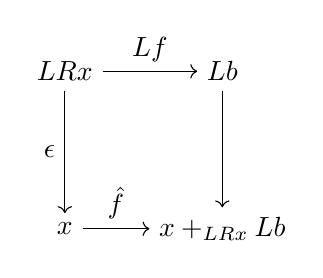
\begin{tikzpicture}
		\node (ul) at (0,2) {$ LRx $};
		\node (ll) at (0,0) {$ x $};
		\node (ur) at (2,2) {$ Lb $};
		\node (lr) at (2,0) {$ x +_{LRx} Lb$};
		\draw [->] (ul) to node [left] {$ \epsilon $} (ll);
		\draw [->] (ul) to node [above] {$ Lf $} (ur);
		\draw [->] (ll) to node [above] {$ \hat{f} $} (lr);
		\draw [->] (ur) to (lr);
	\end{tikzpicture}
	\] 
	Observe that $ R \hat{f} \from Rx \to R( x +_{LRx} Lb ) $. Also there is a string of isomorphisms  
	\[
		R( x +_{LRx} Lb ) \to Rx +_{RLRx} RLb \to Rx +_{Rx} b \to b
	\]
	whose composite we call $ h $. Then $ R \hat{f} = f . h^{-1} $ as desired.  \emph{(note: some details are needed here)}
	
	Now show that $ \hat{f} $ is cocartesian.  Consider a $ \ca{D} $-arrow $ g \from x \to y $ with a $ C $-arrow $ \theta \from R( x +_{LRx} Lb ) \to Ry  $ so that $ R \hat{f} . \theta = Rg $.  Can we uniquely lift $ \theta $? Set up the diagram
	\[
	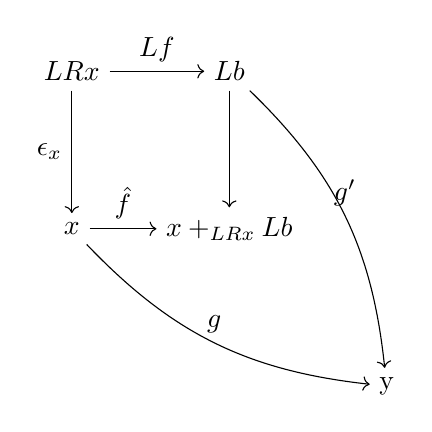
\begin{tikzpicture}
		\node (ul) at (0,2) {$ LRx $};
		\node (ll) at (0,0) {$ x $};
		\node (ur) at (2,2) {$ Lb $};
		\node (lr) at (2,0) {$ x +_{LRx} Lb$};
		\node (comp) at (4,-2) {y};
		\draw [->] (ul) to node [left] {$ \epsilon_x $} (ll);
		\draw [->] (ul) to node [above] {$ Lf $} (ur);
		\draw [->] (ll) to node [above] {$ \hat{f} $} (lr);
		\draw [->] (ur) to (lr);
		\draw [->] (ll) to [bend right=20] node [above] {$ g $} (comp);
		\draw [->] (ur) to [bend left=20] node [above] {$ g' $} (comp);
	\end{tikzpicture}
	\] 
	where $ g' \bydef Lh^{-1} . L\theta.\epsilon_y $.  To show the outer square commutes, it suffices to show that $ Lf . g' $ and $ \epsilon_x . g $ have the same image under the adjunction homset correspondence.  We have
	\[
		Lf . g' = Lf . Lh^{-1} . L\theta.\epsilon_y 
			\mapsto \eta_{Rx} . RLf . RLh^{-1} . RL\theta.R\epsilon_y 
			= f . h^{-1} . \theta  
			= R \hat{f} . \theta 
			= Rg
	\]
	and 
	\[
	\epsilon_x . g \mapsto \eta_{Rx} . Rg = Rg.	
	\]
\end{proof}



\begin{thm}
	Given a Street opfibration $ R \from \ca{D} \to \ca{C} $, it is a right adjoint when it is nice.
\end{thm}
 
Let's try to figure out what nice could be. Here are some helpful theorems.

\begin{thm}[Freyd's general adjoint functor theorem]
\label{thm:GAFT}
	A functor $ F \from X \to Y $ is a right adjoint if  $ x $ is complete, locally small, and $ F $ satisfies the \emph{solution set condition}. The latter says, for any $ Y $-object $ y $, there exists a small set $ I $ indexing a collection of $ X $-objects $ {x_i}_I $ and $ Y $-arrows $ {f_i \from y \to F ( x_i ) } $ such that every $ F $-valued $ Y $-arrow $ y \to R x $ factors as $ Fg . f_k $ for $ k \in I $ and $ g \from x_k \to x $.
\end{thm}

\begin{proof}
	The proof is V.6.2 in CWM.  Define the left adjoint $ G \from Y \to X $ by $ G (y) \coloneqq x $ where $ y \to F x $ is initial in the comma category $ y \downarrow F $.  
\end{proof}

\begin{thm}[Gabriel-Zisman]
\label{thm:GabZis}
	An adjunction $ L \dashv R \from \ca{C} \leftrightarrow \ca{D} $. TFAE:
	\begin{enumerate}
		\item $ L $ is full and faithful;
		\item the unit is an isomorphism;
		\item the induced comonad on $ \ca{D} $ is idempotent, $ L $ is conservative, and $ R $ is essentially surjective.
	\end{enumerate}
\end{thm}

Now, let's prove a strong theorem then try to weaken it

\begin{thm}
	Let $ \ca{D}$ be locally small and complete. Also let $ R \from \ca{D} \to \ca{C} $ be a continuous, surjective-on-objects Grothendiek opfibration.  Then $ R $ is a right adjoint.
\end{thm}

\begin{proof}
	We use \ref{thm:GAFT}.  Suffice to show the solution set condition holds.  Fix a $ C $-objects $ c $.  Then the indexing set is $ \ast $, the collection of $ D $-objects consists of a single object $ x_c $ over $ c $ (which exists by surjective-on-objects assumption), and the collection of $ \ca{C} $-arrows consists of the identity.  Any map $ f \from c \to Rd $ has a cocartesian lifting $ \hat{f} \from x_c \to x_{Rd} $ and $ f = R \hat{f} . 1_c $.
\end{proof}

\begin{thm}
	Let $ \ca{D}$ be locally small and complete. Also let $ R \from \ca{D} \to \ca{C} $ be a continuous, surjective-on-objects, conservative Street opfibration.  Then $ R $ is a right adjoint.
\end{thm}

\begin{proof}
	We use \ref{thm:GAFT}.  Suffice to show the solution set condition holds.  Fix a $ C $-objects $ c $.  Then the indexing set is $ \ast $, the collection of $ D $-objects consists of a single object $ x_c $ over $ c $ (which exists by surjective-on-objects assumption), and the collection of $ \ca{C} $-arrows consists of the identity.  For any map $ f \from c \to Rd $, there exists an essential cocartesian lifting $ \hat{f} \from x_c \to d' $ together with a $ \ca{C} $-isomorphism $ h \from Rd' \to Rd $ such that $ f = h . R \hat{f} $. But $ f = h . R \hat{f} = R \hat{h} . R \hat{f} . 1_c = R (\hat{h} . \hat{f}) . 1_c $ where $ h = R \hat{h} $ because $ R $ is conservative.
\end{proof}

\begin{thm}
	Let $ \ca{D}$ be locally small and complete. Also let $ R \from \ca{D} \to \ca{C} $ be a continuous, essentially surjective, conservative Street opfibration.  Then $ R $ is a right adjoint.
\end{thm}

\begin{proof}
	We use \ref{thm:GAFT}.  Suffice to show the solution set condition holds.  Fix a $ C $-object $ c $.  Then the indexing set is $ \ast $, the collection of $ D $-objects consists of a single object $ d' $ where $ \theta \from c \cong Rd' $ (which exists by essential surjectivity), and the collection of $ \ca{C} $-arrows is $ { \theta } $.  For any $ \ca{C} $-arrow $ f \from c \to Rd $, we have (by Street opfibrationness) $ f . \theta^{-1} \from Rd' \to c \to Rd $, a cocartesian essential lifting $ \hat{ f . \theta^{-1} } \from d' \to d'' $ in $ \ca{D} $, and an isomorphism $ h \from d \to d'' $ (by conservatism) such that $ f . \theta^{-1} = Rh . R \hat{ f . \theta^{-1} } $.  This implies, as required by GAFT, that $ f = R (h\hat{ f . \theta }) . \theta $.
\end{proof}

Thoughts about these assumptions. Here are the desired examples I can think of now: $ \ca{Set} $ together with $ \ca{Graph} $ or $ \ca{Top} $. The enriched over sets and completeness are both there. So is essential surjectivity. And reflection of isomorphisms.  The continuity is definitely needed, since it's necessary if $ R $ is a right adjoint. 

Go back to the right adjoint we had in the ``converse'' to the above theorem.  That is, we have a coreflection $ L \dashv R \from \ca{C} \leftrightarrow \ca{D} $ where $ L $ is left exact.  Of course this gives the continuity of $ R $. Essential surjectivity follows from Gabriel-Zisman. Is it a Street opfibration? $ L $ is conservative, but is $ R $?

\begin{ex}
	No, $ R $ is not in general conservative.  Consider the underlying node functor $ \Grph \to \Set $.  All $ \Grph $-endomorphisms on
	\[
	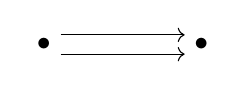
\begin{tikzpicture}
		\node (a) at (0,0) {$ \bullet $};
		\node (b) at (2,0) {$ \bullet $};
		\draw [->] (a.30) to (b.150);
		\draw [->] (a.-30) to (b.-150);
	\end{tikzpicture}
	\]
	are sent to the identity on $ 2 $.
\end{ex}

At this point, we have partial converses:

\fbox{
\begin{minipage}{0.4\textwidth}
		Let $ \ca{D} $ have pushouts. Given a coreflection $ L \dashv R \from \ca{C} \to \ca{D} $ where $ R $ preserves pushouts, $ R $ is a Street opfibration.
\end{minipage}
}
\hfill
\fbox{
\begin{minipage}{0.4\textwidth}
		Let $ \ca{D}$ be locally small and complete. Also let $ R \from \ca{D} \to \ca{C} $ be a continuous, essentially surjective, conservative Street opfibration.  Then $ R $ is a right adjoint.
\end{minipage}
}

\section{Categories of fibrations and adjunctions}

The key players here are subcategories of $\OpFib$ of those opfibrations that are fibred cocomplete, and of something like
$\Rali$ of ralis that strictly preserve all colimits.

{\chris Also, not sure if separate section for that, but we should try and include as many reasonable examples as possible. The quality rather
than the quantity is important I think! Grph Set the first such.}

\bibliographystyle{alpha}
\bibliography{references}



\end{document}

